\chapter{Videojuego basado en agentes}

\begin{figure}[h]
	\centerline{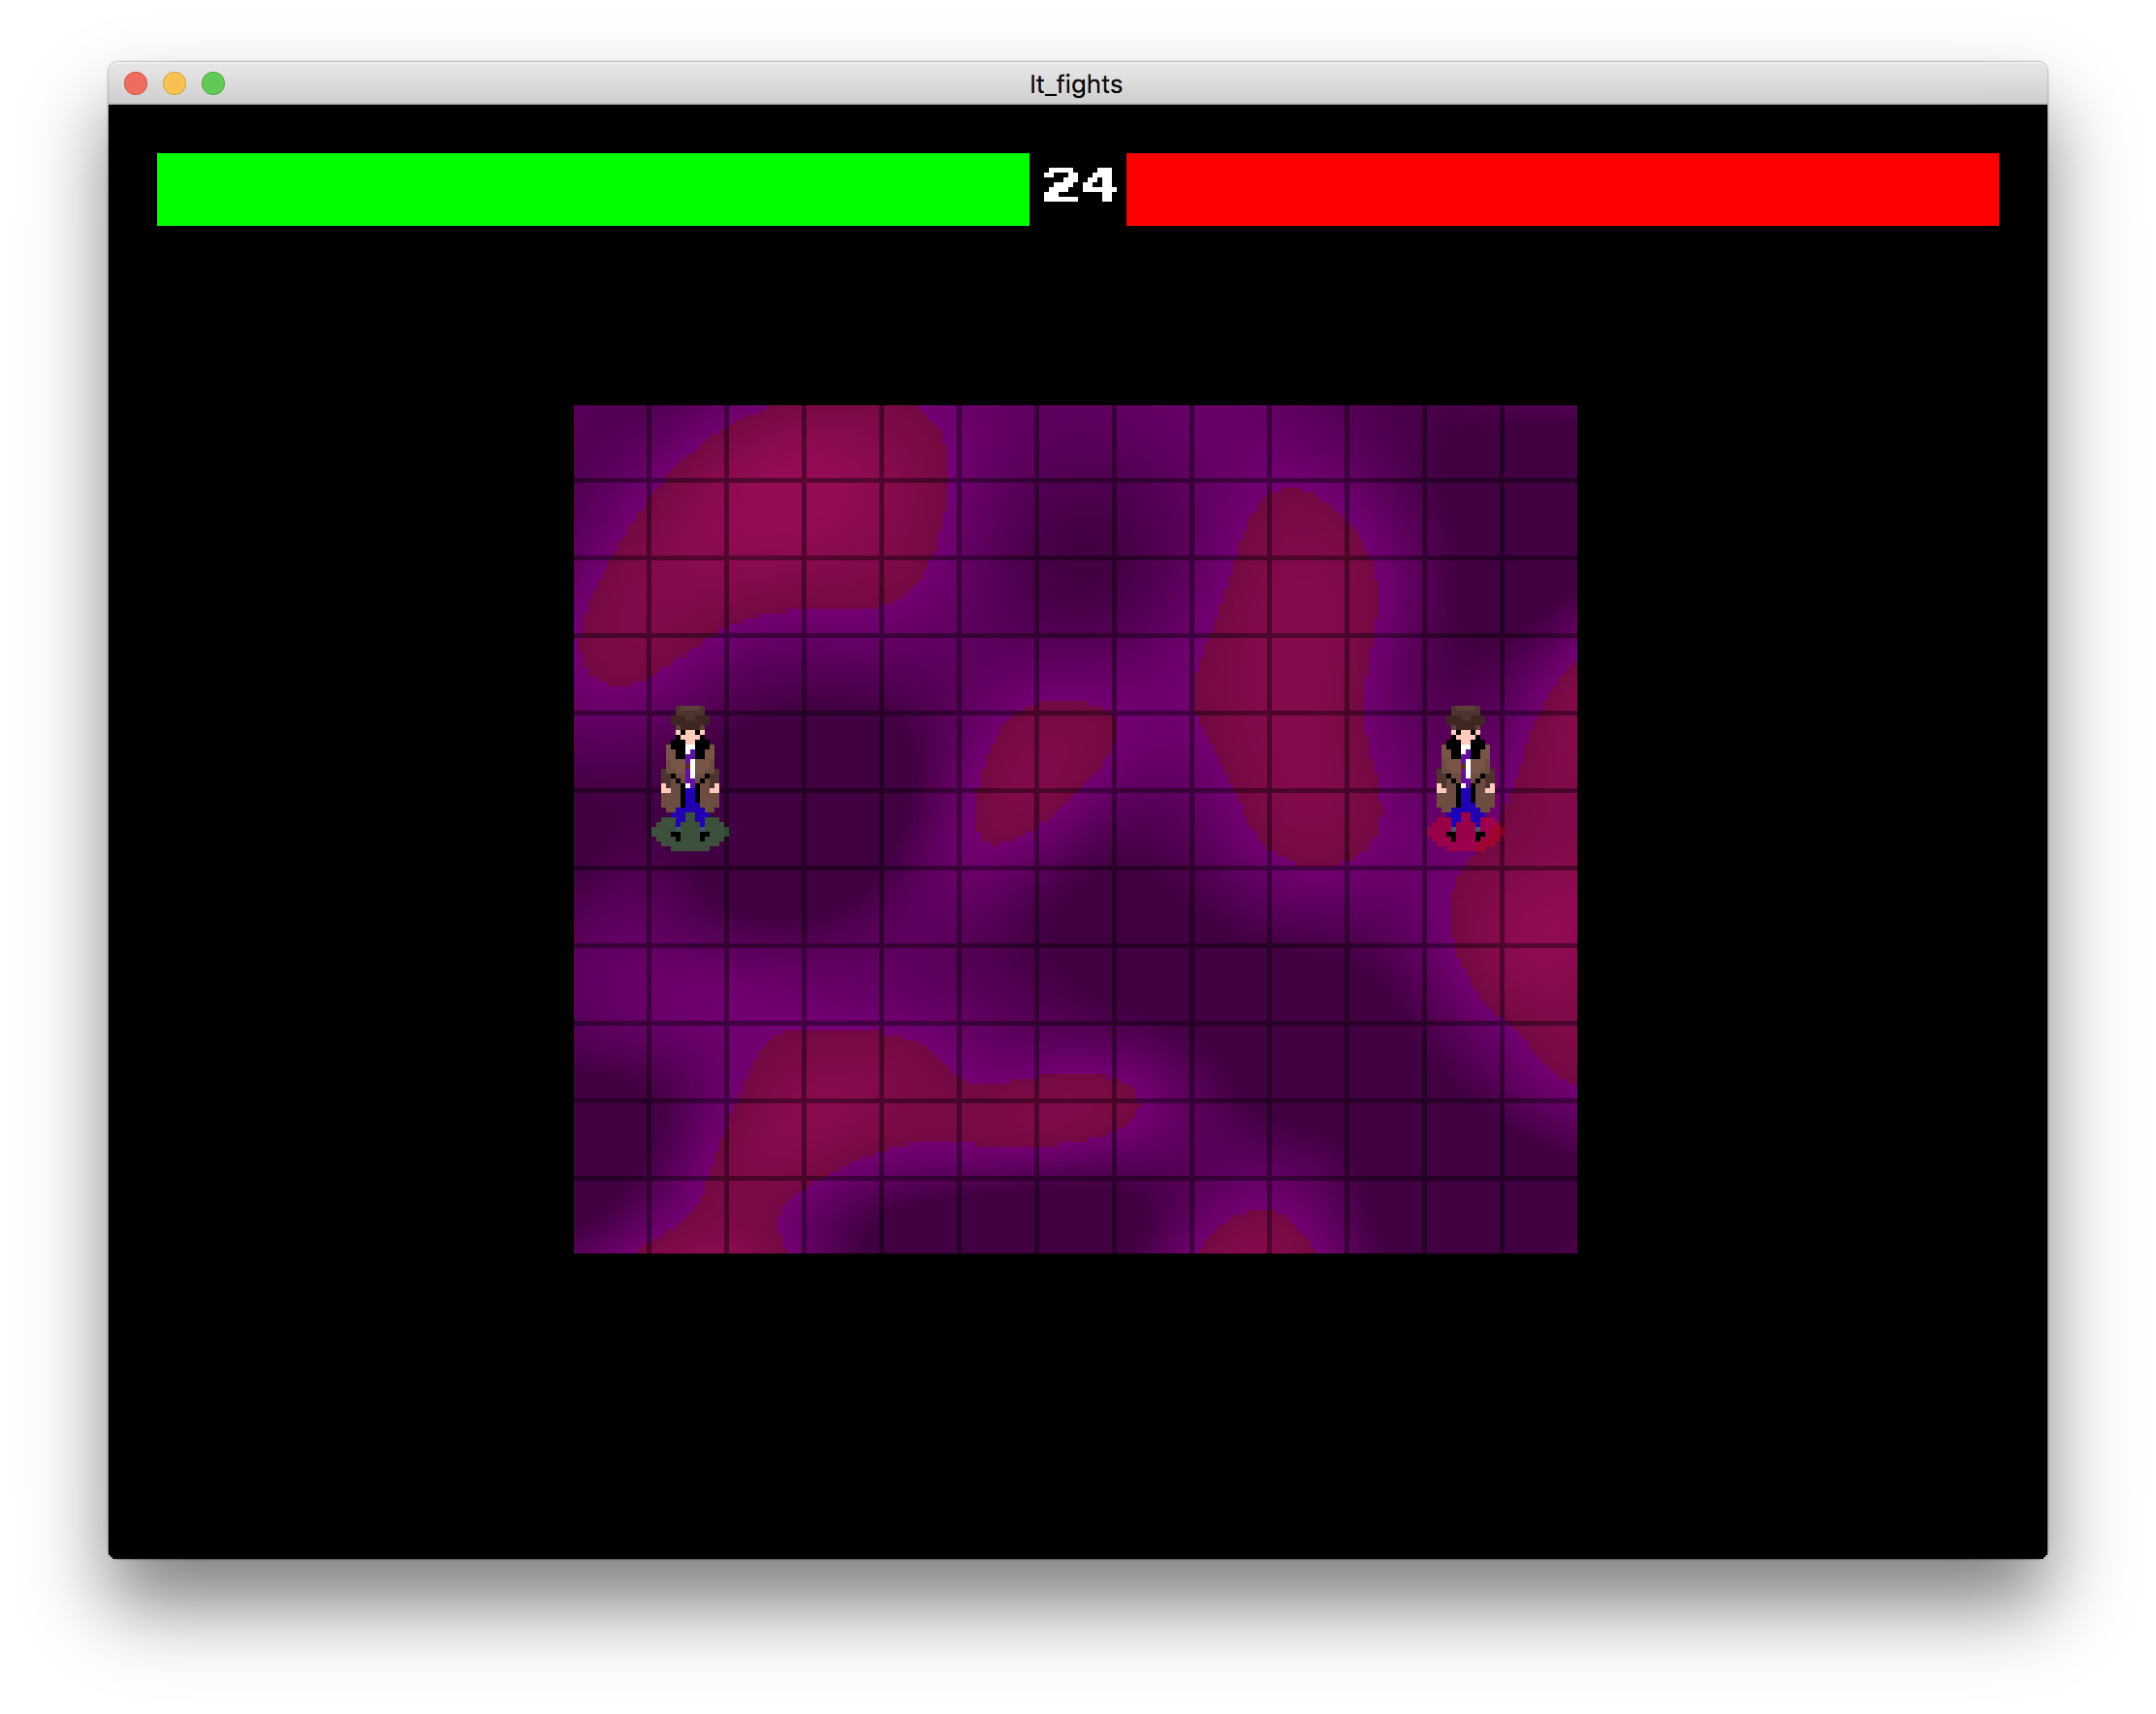
\includegraphics[width=12.5cm]{otros/manual/pelea1.png}}
	\caption{Escena de combate}
	\label{ejemploVideojuego}
\end{figure}

Las \textbf{mecánicas} presentes en el videojuego han sido diseñadas buscando un número reducido pero que aporten cierta profundidad al combate. La figura \ref{ejemploVideojuego} muestra una captura de un combate que sirve como soporte para comprender las mecánicas explicadas a continuación.

\bigskip

Un personaje puede moverse libremente por la zona de combate que se limita por cuatro paredes (habitación rectangular). Además podrá atacar en la zona justo enfrente de él y defenderse de ataques que vienen desde cualquier dirección. Se explican las interacciones entre mecánicas en las siguientes líneas:

\begin{itemize}
	\item \textbf{Movimiento}: El hecho de moverse libremente en una área limitada hace que se genere naturalmente la necesidad de evitar situaciones en las que no se pueda escapar del contrincante. De forma similar al \textit{control del ring} en boxeo, es necesario tener hacia donde moverse si se requiere por lo que se añade la complejidad de evitar quedar atrapado entre los muros y el enemigo. Además la única forma de cambiar el ángulo hacia el que se está mirando es moverse hacia esa dirección.
	\item \textbf{Ataque}: Al poder atacar simplemente en la zona directamente enfrente del personaje se hace relevante la dirección hacia la que el mismo está mirando. Pese a que pueda parecer baladí esto hace que se beneficie una actitud agresiva al tener que moverte hacia la dirección del enemigo justo antes de atacar para estar mirando en su dirección.
	\item \textbf{Defensa}: Existe la posibilidad de ejecutar un movimiento defensivo que protege del ataque. Es la maniobra que representa un alto riesgo pero una alta recompensa ya que si se consigue defenderse de un ataque se proporciona la posibilidad de realizar un ataque propio sin consecuencias. Por otro lado, si la defensa no recibe ataques se entra en un periodo de descanso o \textit{cooldown} en el que el personaje es vulnerable.
\end{itemize}

\bigskip

La interacción entre movimiento, defensa y ataque crea situaciones en las que no está determinada la mejor estrategia claramente. Un estilo agresivo es castigado por un estilo defensivo, el estilo defensivo pierde ante un jugador pasivo que simplemente espera a que se entre en la fase vulnerable de la defensa y a su vez el jugador pasivo perderá ante uno agresivo. La clásica fórmula de \textit{piedra-papel-tijeras} aplicada de un contexto continuo ha probado ser efectiva en diseño de videojuegos desde el nacimiento de la industria.

\section{Prototipo de Unity}


La primera implementación se decidió realizar en un motor considerado el estándar de facto para videojuegos de este tamaño, especialmente cuando obtener una versión funcionar rápidamente es una necesidad. En los primeros prototipos se le dio prioridad a probar si el videojuego era capaz de realizar simulaciones con el tiempo acelerado para permitir que el agente aprendiera rápidamente. 

\bigskip

En el primer prototipo que se probó se vio que el motor no era capaz de escalar el paso del tiempo sin que dejaran de funcionar aspectos muy necesarios del mismo. De forma efectiva se tuvo que lidiar con un riesgo que tuvo un impacto relevante en el proyecto, la gestión del riesgo está definida formalmente en la sección \ref{AC}.

\bigskip

En la figura \ref{unity:combate} podemos observar una captura del prototipo. En este caso se observan las vallas pensadas para limitar el área de combate. Las mismas cuentan con atributos que hacen que generen colisiones, es decir, que los personajes no puedan atravesarlas en ningún caso.

\bigskip

\begin{figure}
	\centerline{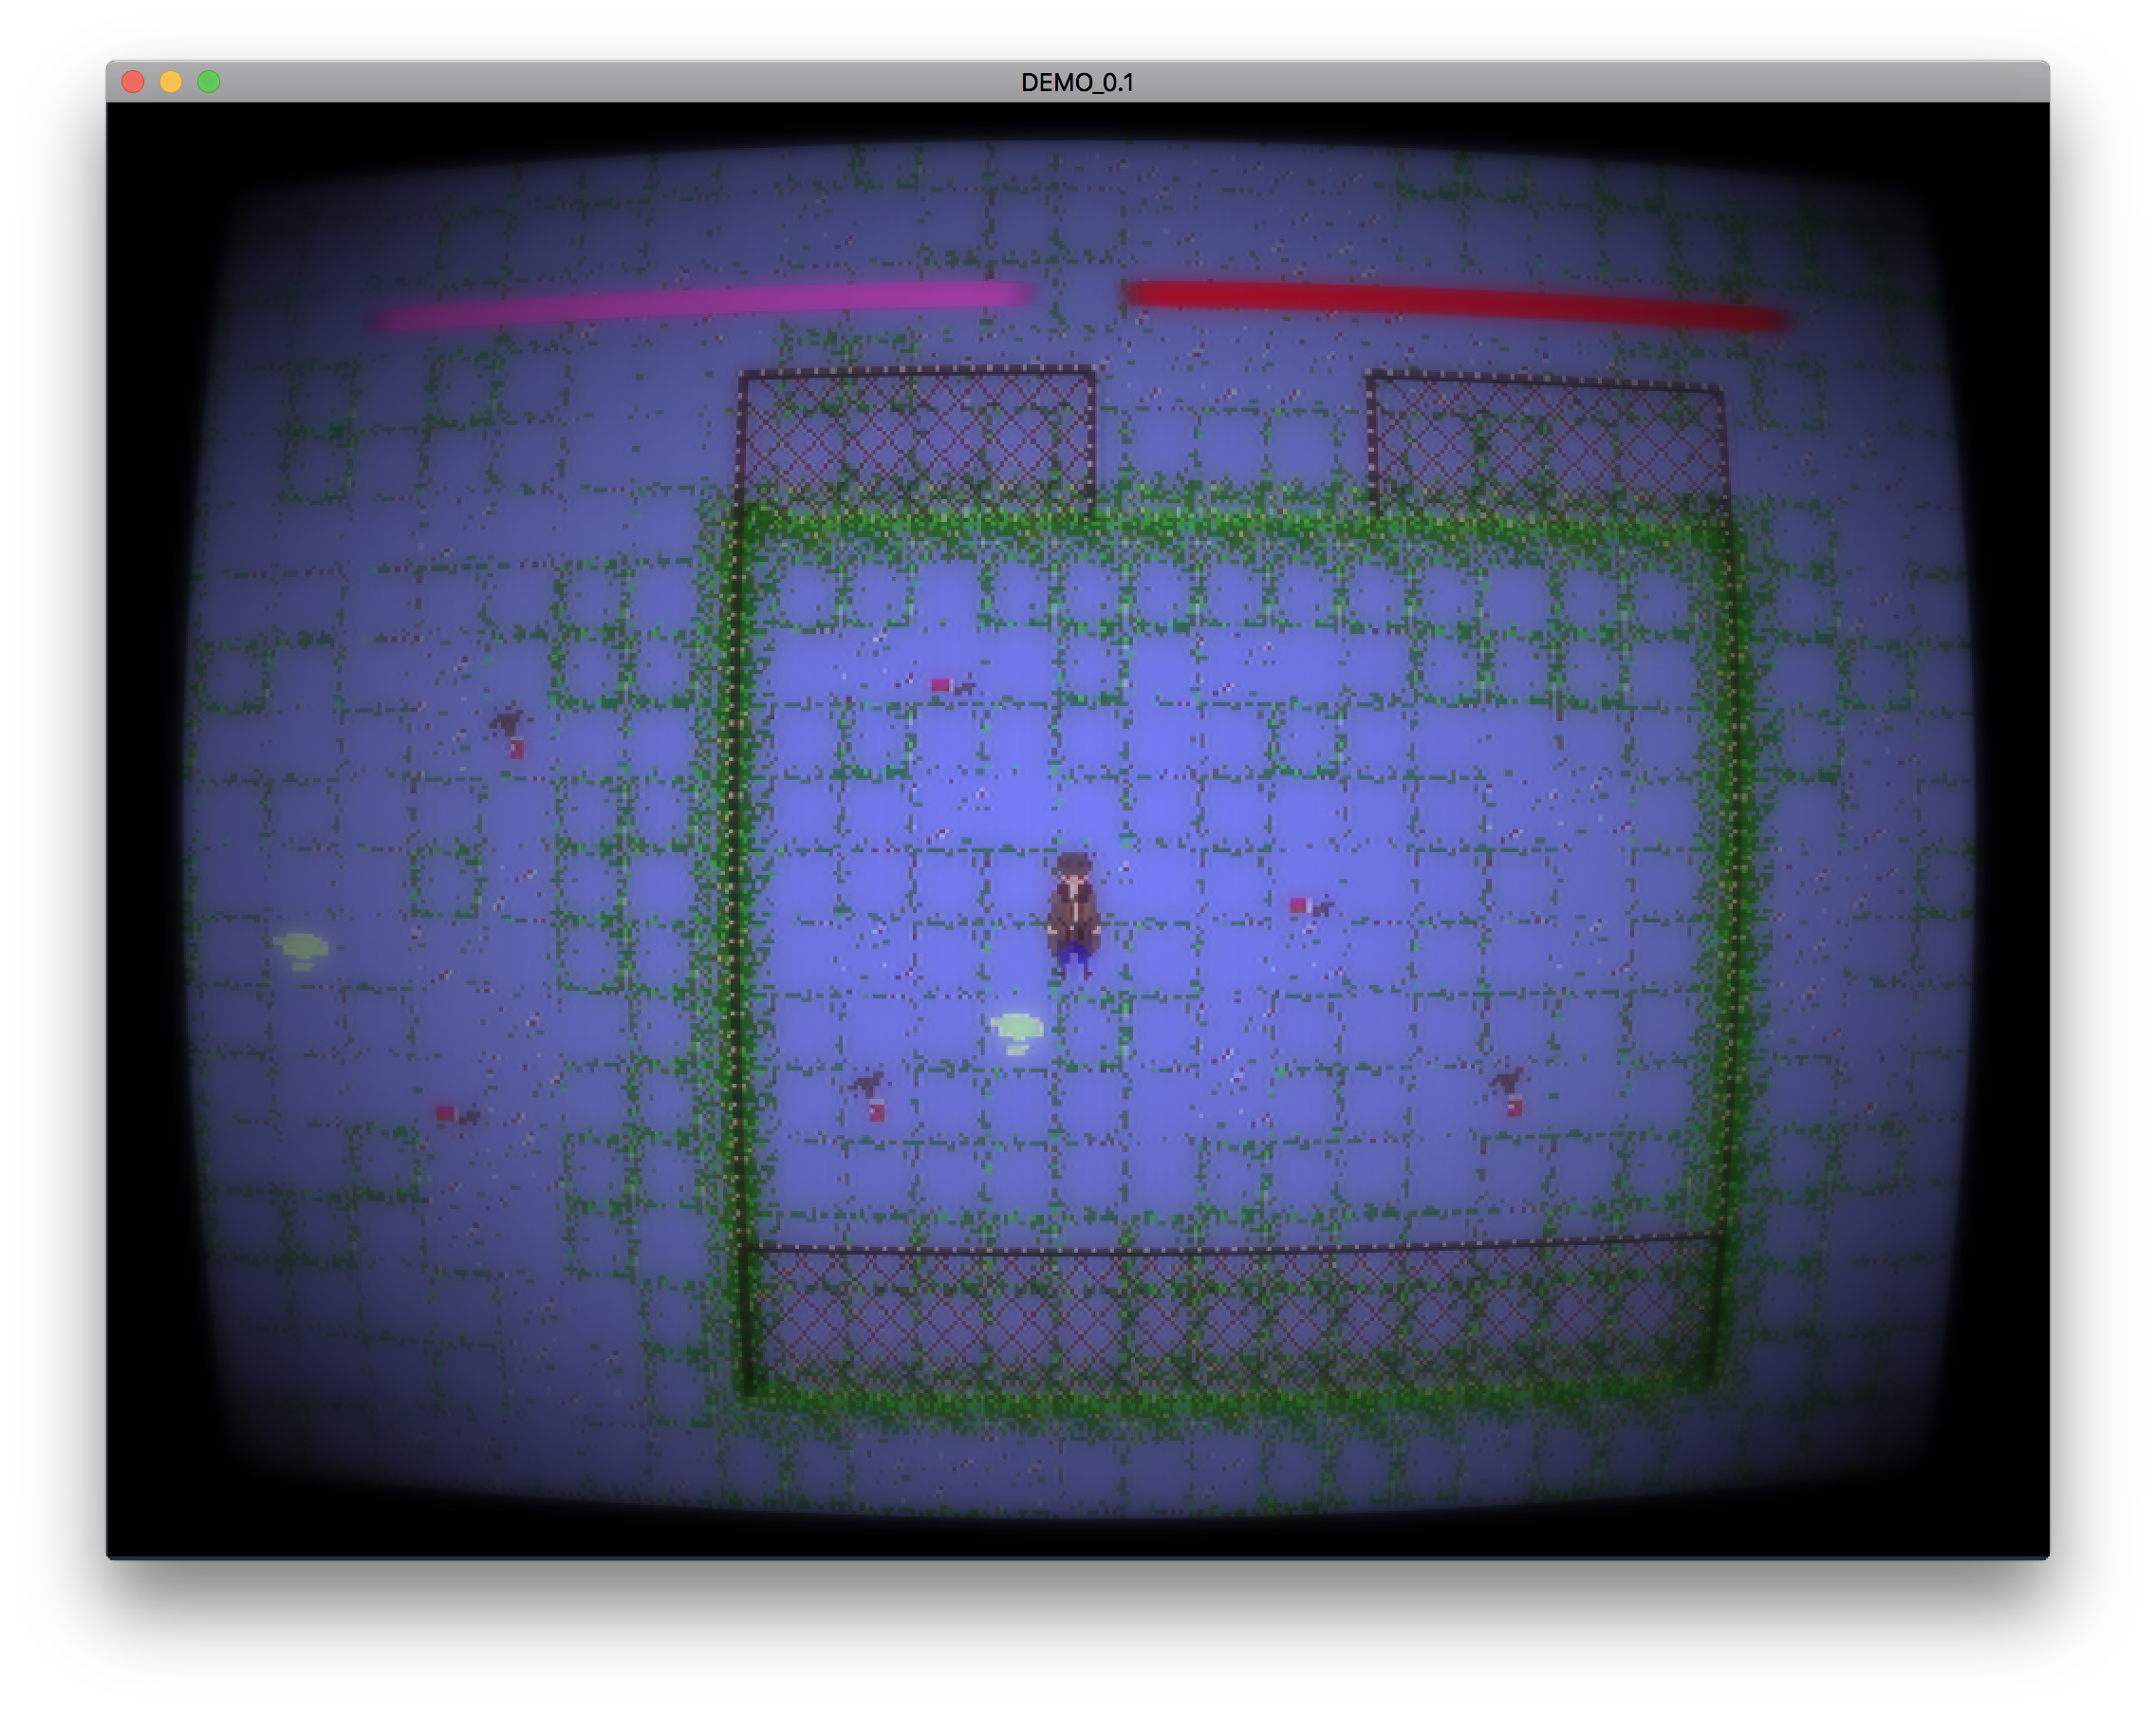
\includegraphics[width=12cm]{otros/otrasCapturas/valla1.png}}
	\caption{Captura del prototipo en la zona de combate}
	\label{unity:combate}
\end{figure}

Sin embargo, al escalar el tiempo por valores relativamente pequeños, este tipo de funcionalidades dejan de funcionar ya que el motor tarda demasiado en componer cada uno de los fotogramas, haciendo que en muchas ocasiones en un fotograma se calcule que el personaje está en un lado de la valla y en el siguiente esté en el otro sin haber entrado en contacto con la misma.

\bigskip

Este tipo de fallos son inaceptables ya que rompen el funcionamiento de las mecánicas de juego al realizar las simulaciones, haciendo que un posible agente no pudiera aprender de forma eficaz y eficiente.

\bigskip

Algo parecido sucede con los ataques. Al intentar acelerar el tiempo y realizar un ataque ocurre con cierta frecuencia que el motor se salta los fotogramas en los que realmente se está comprobando si se hace daño al enemigo, inutilizando esta mecánica también.

\bigskip

En aras de permitir una visualización más comprensible de los problemas se pone a disposición un vídeo en \textit{YouTube}\footnote{Disponible en: \url{https://youtu.be/PY4H8dk8zcU}} en el que se muestra concretamente el problema de la valla. Es cierto que en este caso sí se está mostrando la aplicación y no se está eliminando la visualización para aumentar el rendimiento, sin embargo se ha comprobado que los problemas son los mismos incluso sin visualización. Además el tiempo solo está escalado 20 veces, lo que se esperaría que fuera soportable para el motor pero no es así. Como comparación, en el producto final se escala unas 600 veces sin problema alguno.

\section{Segunda aplicación}

Los problemas mencionados hicieron que se optara por implementar un motor desde cero, lo que aporta control completo sobre el comportamiento de la aplicación y más flexibilidad para enfocarse en los aspectos necesarios para cumplir nuestros objetivos. El diagrama de bloques simplificado mostrado en la figura \ref{bloques} muestra los diferentes componentes que se han creado.

\bigskip

\begin{figure}
	\centerline{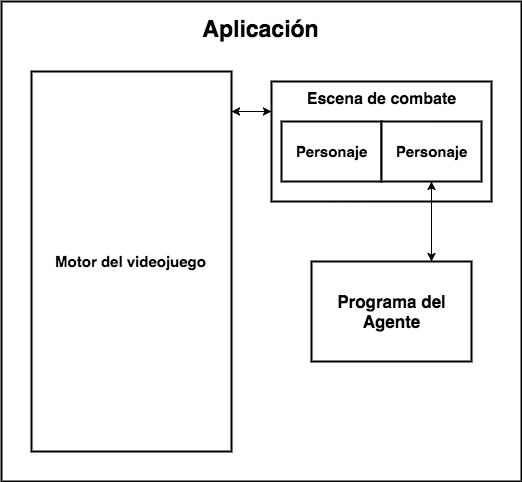
\includegraphics[width=10cm]{otros/otrasCapturas/block.png}}
	\caption{Diagrama de bloques}
	\label{bloques}
\end{figure}


El bloque del motor contiene toda la funcionalidad general necesaria para ejecutar la aplicación, esto incluye todos los subsistemas necesarios para mostrar por pantalla el videojuego, reproducir sonidos, gestionar entrada del usuario, ejecutar las escenas, etc. Se entrará en más detalle en el capítulo \ref{cap:diseno}.

\bigskip

La escena representa el contexto de combate, en el que tendremos dos personajes. La figura, a modo de ejemplo, muestra que uno de ellos está siendo controlado por el agente. El programa del agente es el que contiene las diferentes funcionalidades implementadas para lograr el comportamiento deseado. La siguiente sección, dedicada al algoritmo, entra más en detalle sobre como se han afrontado estas necesidades.


\section{Algoritmo}

El algoritmo implementado recuerda ligeramente a una versión muy simplificada de \textit{Q-Learning}\footnote{Explicación simple de \textit{Q-Learning} en:  \url{http://mnemstudio.org/path-finding-q-learning-tutorial.htm}}. Dada la acción correctiva mostrada en el apartado \ref{AC} se ha optado por una aproximación específica para el problema actual en lugar de realizar implementaciones desde cero de técnicas de aprendizaje por refuerzo. Las mismas requerirían una cantidad de tiempo y recursos del que no se disponía en el proyecto, sin embargo, en el apartado de conclusiones y posibles ampliaciones (\ref{cap:conclusiones}) se especifican las técnicas que sería posible agregar sin demasiado esfuerzo adicional.

\bigskip

{Tipo de red neuronal artificial entrenado para representar de forma discreta un espacio de entrada de estados continuos}. Se ha optado por una discretización manual en la cual los estados continuos del combate generan una estructura que tiene en cuenta los siguientes datos:

\begin{itemize}
	\item \textbf{Vida de los personajes} (6 valores): desde 0 (vacía) hasta 5 (completa).
	\item \textbf{Acción que se está realizando} (5 valores): Que puede ser moverse, atacar, defender, estar quieto o estar descansando de una defensa.
	\item \textbf{Dirección relativa de los personajes} (4 valores): Se calcula la dirección del enemigo de forma discreta (hacia arriba, abajo, izquierda o derecha).
	\item \textbf{Distancia entre los personajes} (3 valores): Que se subdivide en tres estados dependiendo del rango de ataque: fuera de rango, cerca de rango o dentro de rango.
	\item \textbf{Posición de los muros} (9 valores): Se guarda si hay algún muro al lado del personaje que impida su movimiento.
	\item \textbf{Si se está mirando al enemigo} (2 valores): Indica si se está mirando en la dirección del enemigo para poder atacarlo.
\end{itemize}

Dado que la salud y acción realizada se deben guardar para ambos personajes, el número total de estados posibles será:
\bigskip

$(6\times6)\times(5\times5)\times4\times3\times9\times2=194400$

Aunque se ha observado que muchos de ellos son extremadamente infrecuentes pese a simular combates durante decenas de miles de iteraciones.



\subsection{Utilidad o \textit{fitness}}

Una vez discretizados los estados se puede proceder a definir cómo el agente los irá explorando, además de la manera de asociar una recompensa a la mejor acción para cada estado. Para ello se necesita una función de utilidad o \textit{fitness} que se define teniendo en cuenta:

\begin{itemize}
	\item \textbf{Distancia al enemigo}: Se recompensa al personaje cuando se acerca al enemigo para favorecer un comportamiento agresivo.
	\item \textbf{Vida propia del enemigo}: Se recompensa al personaje cuanta más vida tenga y cuanta menos tenga el enemigo.
	\item \textbf{Posición de los muros}: Se recompensa al personaje si no está al lado de ningún muro que impida el movimiento en esa dirección.
	\item \textbf{Si se está mirando al enemigo}: Se recompensa al personaje si está mirando al enemigo ya que esto posibilita realizar un eventual ataque exitoso.
\end{itemize}

\bigskip

En concreto, el valor de \textit{fitness} de cada estado se calculará siguiendo el algoritmo \ref{algoritmo:fitness}. En el mismo se puede observar cómo se comienza con un valor inicial y luego se irán sumando o restando según si las variables utilizadas se consideran directamente o inversamente proporcionales al valor de \textit{fitness} deseado.

\bigskip

Es importante considerar los valores de los \textbf{\textit{BONUS}} y \textbf{\textit{MULTIPLICADORES}} que se usan para calcular las variables ya que al cambiarlos se le dará más o menos importancia a la variable que modifican.

\bigskip

El cuadro \ref{algoritmo:valores} contiene los valores utilizados en la versión final del proyecto que han sido obtenidos para intentar maximizar la agresividad del jugador. Los valores introducidos han surgido de una observación iterativa del \textit{fitness} que se asociaba a estados en los que se encontraba el personaje controlado por el jugador. En cada caso concreto se ha determinado si la variación de \textit{fitness} era la correcta para cada estado teniendo en cuenta el comportamiento ideal deseado para el agente.

\bigskip

Una vez que se determinaron valores aparentemente válidos a ojos del desarrollador se comenzó con la etapa de entrenamiento la cual, con sus buenos resultados, demostró que esas cantidades eran apropiadas.

\bigskip

\begin{table}
	\begin{center}
		\begin{tabular}{|l|l|}
			\hline
			\textbf{Parámetro} & \textbf{Valor}\\
			
			\hline
			INITIAL\_FITNESS\_VALUE& 1000\\
			
			\hline
			MY\_HEALTH\_MULTIPLIER& 100\\
			
			\hline
			ENEMY\_HEALTH\_MULTIPLIER& 100\\
			
			\hline
			DISTANCE\_MULTIPLIER& 3\\
			
			\hline
			LOOKING\_BONUS& 200\\
			
			\hline
			WALL\_BONUS& 50\\
			
			\hline
		\end{tabular}
		\caption{Valores utilizados en la función de \textit{fitness}}
		\label{algoritmo:valores}
	\end{center}
\end{table}


\begin{algorithm}
	
	\SetKwData{Fitness}{fitness}
	
	\SetKwData{PlayerHealth}{playerHealth}
	\SetKwData{EnemyHealth}{enemyHealth}
	\SetKwData{Distance}{distance}
	\SetKwData{LookingAtEnemy}{lookingAtEnemy}
	\SetKwData{NoWallsNear}{noWallsNear}
	
	\SetKwFunction{GetRandomAction}{getRandomAction}
	\SetKwInOut{Input}{input}\SetKwInOut{Output}{output}
	\Input{\PlayerHealth, \EnemyHealth, \Distance, \LookingAtEnemy, \NoWallsNear}
	\Output{\Fitness}
		
		
		\Fitness$\leftarrow$ INITIAL\_FITNESS\_VALUE\;
		\Fitness$\leftarrow$ \Fitness$+ ($\PlayerHealth$*$ MY\_HEALTH\_MULTIPLIER$)$\;
		\Fitness$\leftarrow$ \Fitness$- ($\EnemyHealth$*$ ENEMY\_HEALTH\_MULTIPLIER$)$\;
		\Fitness$\leftarrow$ \Fitness$- ($\Distance$*$ DISTANCE\_MULTIPLIER$)$\;
		
		\If{\LookingAtEnemy}{
			\Fitness$\leftarrow$ \Fitness$+$ LOOKING\_BONUS\;
		}
	
		\If{\NoWallsNear}{
			\Fitness$\leftarrow$ \Fitness$+$ WALL\_BONUS\;
		}

	\caption{Algoritmo de cálculo de \textit{fitness}}
	\label{algoritmo:fitness}
\end{algorithm}

\bigskip


\bigskip

Por otra parte, las acciones discretas que puede realizar el jugador son sencillas: Atacar, defenderse, moverse en cuatro direcciones (arriba, abajo, izquierda o derecha) o quedarse quieto.


\subsection{Aprendizaje}

Ahora que se cuenta con una función de utilidad, estados discretos y acciones discretas se procede a definir cómo el agente aprende y escoge entre las diferentes opciones en el \textbf{algoritmo} \ref{algoritmo}.

\bigskip


En el mismo se muestra cómo en cada iteración del bucle que ejecuta el agente primero se guardará la información referente al estado anterior, la acción elegida y la mejora en \textit{fitness} asociada. Después de esto se escogerá o bien una acción aleatoria si no se conoce el estado o una de entre las posibles que se ha observado con una probabilidad proporcional a su \textit{fitness}.

\bigskip


\textbf{$\epsilon$} representa una cantidad entre 0 y 1 que indica que porcentaje de las veces que se elige sobre un estado conocido se decide explorar un estado aleatorio en lugar de  elegir uno de los visitados. Se han utilizado valores cercanos a $0.30$ durante el entrenamiento y se han disminuido a valores ligeramente menores a $0.1$ al finalizar el mismo con la intención de comprobar sus habilidades.

\bigskip

El algoritmo se ejecutará una vez por cada ciclo de actualización del agente, o lo que es lo mismo, del personaje que controla. De esta forma, cada vez que se hace la llamada al \textit{update} del agente se realiza un ciclo del algoritmo \ref{algoritmo}. Para comprender la estructura de los objetos que representan el capítulo \ref{cap:diseno} puede ser de ayuda, especialmente la sección \ref{cap:diseno:agente}.

\bigskip

En la aplicación se permite que el agente compita contra el mismo, de forma que controla a los dos personajes a la vez. A ojos del agente es irrelevante cual o cuantos personajes tiene que considerar, simplemente recibe estados, un fitness asociado e intenta elegir la acción correcta.

\bigskip

Esta aproximación permite realizar un entrenamiento el doble de rápido tal y como se muestra en la sección \ref{cap:pruebas:mismo}. Sin embargo, a cambio de esto se pierde la posibilidad de enfrentar a dos agentes que tengan entrenamiento diferente. Esto no ha sido una prioridad ya que se busca un entrenamiento orientado a jugadores reales y a la representación de su comportamiento que compone el personaje basado en reglas.




\begin{algorithm}
	
	\SetKwData{Action}{action}
	\SetKwData{LastAction}{selectedAction}
	\SetKwData{LastState}{lastState}
	\SetKwData{CurrentState}{currentState}
	\SetKwData{DeltaFitness}{deltaFitness}
	\SetKwData{StateActionData}{stateActionData}
	\SetKwData{RandomAction}{randomAction}
	\SetKwData{AllActions}{allPosibleActions}
	
	\SetKwFunction{GetRandomAction}{getRandomAction}
	\SetKwFunction{GetCurrentState}{getCurrentState}
	\SetKwFunction{RandomBet}{randomBetween}
	\SetKwFunction{CalculateFitness}{calculateFitness}
	\SetKwFunction{UpdateWith}{updateWith}
	\SetKwFunction{Insert}{insert}
	\SetKwFunction{Pick}{bestWeightedAction}
	
	\While{agent is running}{
		\LastState$\leftarrow$ \CurrentState\;
		\CurrentState$\leftarrow$ \GetCurrentState{}\;
		
		\DeltaFitness$\leftarrow$ \CalculateFitness{\CurrentState}$-$\CalculateFitness{\LastState}\;
		
		%Actualizamos el conocimiento del agente
		\uIf{\LastState$\in$ \StateActionData}{
			\StateActionData$.$\UpdateWith{\LastState,\LastAction,\DeltaFitness}\;
		}
		\Else{
			\StateActionData$.$\Insert{\LastState,\LastAction,\DeltaFitness}\;
		}
		
		
		%Seleccionamos la acción a escoger
		\uIf{\CurrentState$\in$ \StateActionData}{
			
			\uIf{\RandomBet{$0$,$1$}$<\epsilon$}{
				\LastAction$\leftarrow$ \RandomAction $\in$ \AllActions\;
			}
			\Else{
				\LastAction$\leftarrow$ \Action $\in$ \AllActions  $|$ \Pick{\StateActionData,\CurrentState} $=$ \Action  \;
			}
			
		}
		\Else{
			\LastAction$\leftarrow$ \RandomAction $\in$ \AllActions\;
		}
		
		
	}
	\caption{Algoritmo general del agente}
	\label{algoritmo}
\end{algorithm}

\section{Agente basado en reglas}

Para realizar simulaciones en las que el agente sea capaz de aprender sin la necesidad de tener a un jugador humano combatiendo contra él se ha realizado la implementación de un agente basado en reglas simples que se comporta de una forma definida ante cierto conjunto de estados.

\bigskip

Para componer el conjunto de reglas se han realizado una serie de combates entre jugadores reales para obtener datos sobre cual és la estrategia general seguida por los mismos. A grandes rasgos dicha estrategia involucra comportarse de forma ofensiva cuando se tiene más vida dando más prioridad a la defensa cuando más daño se recibe. Además independientemente de la vida propia, si el enemigo está muy débil se prioriza intentar derrotarlo a escapar.

\bigskip

\begin{table}
	\begin{center}
		\begin{tabular}{|l|l|}
			\hline
			\textbf{Condición} & \textbf{Acción}\\
			
			\hline
			Si la vida del enemigo es muy baja ($\leq2$) & Ataque agresivo\\
			
			\hline
			Si la vida del enemigo es baja ($\leq3$) & Ataque agresivo o Contraataque\\
			
			\hline
			Si la vida propia es muy alta ($\geq4$)& Ataque agresivo\\
			
			\hline
			Si la vida propia es alta ($\geq3$)& Ataque agresivo o Contraataque\\
			
			\hline
			Si la vida propia es baja ($\leq2$) & Ataque defensivo o Escape defensivo\\
			
			\hline
		\end{tabular}
		\caption{Agente basado en reglas}
		\label{reglas}
	\end{center}
\end{table}


La tabla \ref{reglas} resume a alto nivel los comportamientos especificados. Se recorre la tabla de arriba a abajo, ejecutando la acción asociada a la primera condición que se cumpla. Las acciones descritas en la misma tienen el siguiente significado:

\begin{itemize}
	\item \textbf{Ataque agresivo}: Se persigue al oponente hasta que se tiene a un rango en el que se le puede asestar un ataque.
	\item \textbf{Contraataque}: Se hace parecer que se está abordando al oponente con un ataque esperando a que este se defienda, cuando este lo hace se espera a que no se pueda defender y se ataca.
	\item \textbf{Ataque defensivo}: Se escapa del oponente pero si este se encuentra en situación de ser atacado se le intenta asestar un golpe.
	\item \textbf{Escape defensivo}: Se escapa del oponente pero si este intenta atacar al personaje se realizará la maniobra defensiva.
\end{itemize}

En los casos en los que hay varias acciones se escoge una de ellas de forma aleatoria. De este modo se genera un comportamiento que va cambiando entre diferentes combates. De esta forma la variedad en las peleas no solo la aporta el agente que aprende sino el basado en reglas.

\section{Tipos de entrenamiento}


El entrenamiento del agente se puede realizar de varios modos, obteniendo diferentes beneficios de cada uno de ellos. Se seguirán principalmente dos aproximaciones diferentes que son las siguientes:

\begin{itemize}
	\item \textbf{Realizar una serie de combates de forma iterativa contra el agente basado en reglas}: De esta forma se aprenderá un comportamiento simulado relativamente similar al de jugadores reales. Esta aproximación pretende reemplazar el contar con jugadores humanos compitiendo contra el agente durante cientos o miles de iteraciones.
	\item \textbf{Hacer combatir al agente contra otro personaje controlado por él mismo}: Obteniendo una variabilidad en los combates que le permite al agente familiarizarse con situaciones poco comunes. Además se evita que se aprenda un comportamiento óptimo para un tipo de enemigo que no rinda lo suficiente contra otro, algo deseable si se pretende afrontar la variabilidad en comportamiento de un jugador humano. 
\end{itemize}

Se muestra en el apartado de pruebas (sección \ref{sec:valicacion}) cómo se comportan cada uno de los agentes entrenados de estas dos formas únicamente. Para la obtención del agente mostrado en el producto final se ha seguido una combinación entre ambas estrategias, combatiendo primero contra el agente basado en reglas y luego contra él mismo.

\bigskip

De esta forma se aprende rápidamente al principio del entrenamiento pues el entorno competitivo que presenta el agente basado en reglas es significativamente más complejo que el de un agente que no ha aprendido nada. Luego, cuando el agente ya es capaz de pelear, se realizan combates contra él mismo buscando la exploración del máximo numero de situaciones, y por lo tanto estados, que se pueden dar.

\bigskip

Esta exploración de más estados surge de que el comportamiento del agente basado en reglas es limitado comparado con el que aprende siguiendo el algoritmo presentado.


